	\chapter{Rappresentazione in memoria}\label{mem}
	%todo si può fare una sorta di introduzione anche grafica?
	Premessa: questo capitolo ti sembrerà estremamente astratto e fine a se stesso. Non è così, o meglio: è sì astratto, ma è molto utile per poter capire due argomenti decisamente pratici che affronteremo più avanti: gli \emph{array} e i \emph{puntatori} (oltre al fatto che alcune nozioni di questo capitolo sono oggetto dello scritto). In ogni caso, tranquillo: sarà un capitolo breve.\\
	
	
	Qualsiasi programma, per funzionare, deve essere caricato nella memoria. Ricordo che per \emph{memoria} intendiamo la RAM, non il disco fisso. Quando avviamo un programma, il sistema operativo va a leggere il codice eseguibile che è immagazzinato nel disco fisso, pensa quest'ultimo come un deposito dove le informazioni possono essere solo stanziate, ma non ``usate'' in maniera attiva; da lì prende il pacchetto di dati che rappresenta il programma e lo carica sulla RAM, e così il programma diventa ``vivo'', cioè può iniziare a funzionare. \\
	
	
	Piccolo inciso (giusto per curiosità, non sono informazioni necessarie per l'esame): la differenza a livello pratico tra hard disk e RAM è che il primo è molto più lento del secondo. Gli hard disk classici sono composti da dischi di materiale magnetico che girano con una testina che legge i dati. La RAM, invece, è una memoria composta da circuiti a stato solido: è estremamente veloce e, mentre la testina dell'hard disk ha difficoltà a muoversi casualmente da un punto all'altro del disco, i dati sulla RAM possono essere letti in maniera sparsa in modo estremamente rapido: non a caso RAM, significa ``random access memory'', memoria ad accesso casuale. I nuovi dischi a stato solido, gli SSD, sono più veloci rispetto a quelli ``classici'', ma comunque lentissimi a confronto con la RAM.
	
	Questa non è l'unica differenza. L'altra sta nel fatto che l'hard disk, magnetico o a stato solido, non ``perde la memoria'': i dati hanno vita virtualmente infinita. Anche quando viene a mancare la corrente di alimentazione, i dati ``sopravvivono''. Lo stesso non vale per la RAM: quando viene meno la corrente (si spegne il computer), si perdono tutti i dati contenuti.  Infine, gli hard disk possono essere centinaia di volte più capienti della RAM. 
	
	Insomma, tutto ciò per dire che il processore ha accesso diretto alla RAM e non all'hard disk. Possiamo pensare il computer come un cervello: il processore è la parte pensante; la RAM è la memoria a breve termine dove vengono caricati i pensieri e i ragionamenti che la parte pensante elabora; l'hard disk è la memoria a lungo termine a cui la parte pensante fa più fatica ad accedere e su cui non può ``ragionare'', e per farlo deve spostare i pensieri sulla memoria a breve termine. Paragone temerario, ma spero un minimo efficace\ldots

	
	\section{La struttura della memoria}	
	Dovrebbe esserti chiaro, ormai, che in informatica nulla è lasciato al caso. Come fa il processore, una volta caricato un programma, a sapere dov'è? Quando usiamo delle variabili, come fa a sapere dove si trovano nella RAM? Insomma: le moderne RAM spesso superano i 4 gigabyte, e un modesto \textbf{int} da 4 byte come può non perdersi in quel mare di memoria?
	
	\`E semplice! Non devi pensare la memoria come un ``continuo'': visto che siamo Fisici, potremmo dire che la memoria è ``quantizzata''. Esistono pacchetti minimi di memoria che il sistema operativo può gestire: i \emph{byte}. La memoria è organizzata in byte: è divisa in tante cellette, una adiacente all'altra, ognuna grande un byte. \\
	Ogni celletta non è persa nel nulla, ma ha un \emph{indirizzo}. 
	
	Voglio che ti sia chiaro un concetto: le cellette di memoria non sono sparse in modo generico, e non sono neanche poste in maniera ``bidimensionale'': sono come lungo una retta, una dopo l'altra. Ogni celletta di memoria confina solo con altre due celle. Immaginati la RAM come una lunghissima striscia suddivisa in miliardi di caselle (sì, miliardi!: un gigabyte sono più di un miliardo di byte) contigue e ordinate (ordinate? ovvero ognuna con un proprio indirizzo!).
	\subsection{Indirizzi di memoria}
	Ogni cella ha un proprio indirizzo, bene, ma come è fatto? 
	
	Un indirizzo di memoria non è altro che un numero intero che la rappresenta: ad esempio, la prima celletta potrebbe essere $00001$, la seconda subito adiacente $00002$, la terza $00003$ e così via fino ad arrivare $78354$ o addirittura $99999$. Insomma: finché c'è spazio la numerazione continua. Io ho usato interi a cinque cifre, ma se la memoria fosse molto più estesa, perché non spingersi fino a 9, 10, ecc\ldots cifre? Nessuno lo vieta, se non la dimensione dalla RAM e l'architettura della CPU; se sei interessato all'argomento prova a leggere i complementi di questo capitolo (\ref{archCPU}).
	
	Però ho commesso, volontariamente, un ``errore'' per aiutarti a capire. I byte non sono indicizzati in sistema decimale (che io ho usato), ma esadecimale (base 16). 
	
	Quando chiediamo al computer di stamparci l'indirizzo di uno specifico byte, ci viene riportato il numero in base 16: dobbiamo velocemente imparare a contare in sistema esadecimale per risolvere gli esercizi di esame (e capire cosa vogliono dire quegli strani simboli che il computer ci riporta quando lo interroghiamo su un indirizzo).
	
	Ho parlato di simboli perché la base 16 ha bisogno di sedici cifre, ma le cifre decimali sono dieci. Le restanti sei dove le troviamo? Le lettere! Ecco: le ``cifre'' della base sedici sono dieci cifre numeriche e sei lettere. Contiamo da 1 a 16: $0, 1, 2, 3, 4, 5, 6, 7, 8, 9, a, b, c, d, e ,f$.
	
	Se vogliamo scrivere il numero 17 in base esadecimale sarà: 10; 18 diventerà 11 e così via. 
	
	Insomma non ti stupire se trovi numeri di questo tipo: $1a34f2d$. \\
	
	In ``informatica'' i numeri costanti esadecimali,  per contrassegnarli dalle normali stringhe di lettere (e dai numeri in base dieci), iniziano in un modo particolare: $0x\ldots$\\
	Un generico indirizzo di memoria potrebbe essere: $0x7ffd97889f98$ (generico ma sensato: l'ho preso dal mio computer!).

	Abbiamo parlato di questa immaginaria striscia di cellette di memoria da un byte l'una e abbiamo detto che ognuna di loro ha un indirizzo, ecco un'immagine di come puoi pensarla:
	
\begin{figure} [ht]
	\centering
	\includegraphics[scale=0.3]{Immagini/memory.pdf}  
	\captionsetup{justification=centering,margin=2cm}
	\caption{Rappresentazione di un pezzo di memoria: ogni cella, con il relativo indirizzo, rappresenta un byte\protect\footnotemark.}
	\label{memory1}
\end{figure}
\footnotetext{Ringrazio Stefano Balzan per la realizzazione dell'immagine.}
	\section{Stack e Heap}\label{stackheap}
	La RAM è, sul piano logico, suddivisa in due: la \emph{stack} e la \emph{heap}. Si potrebbe dire molto sulle reciproche differenze, ma cercherò di limitarmi alle informazioni che ci saranno utili. 
	
	La \emph{stack} è completamente gestita dal compilatore, e perché ciò avvenga è necessario che la memoria del programma sia già definita a \emph{compile time}, cioè al momento della compilazione. La \emph{stack} è la cosidetta \emph{memoria statica}. 
	
	Quando noi dichiariamo una serie di variabili, per esempio nel \emph{main}, la memoria necessaria è completamente definita al momento della compilazione: se abbiamo dichiarato un \textbf{char} e tre \textbf{int} il compilatore sa che deve riservare un byte per il primo e dodici byte per i secondi. Viene detta \emph{memoria statica} perché non può essere modificata dall'utente a \emph{run time}, durante l'esecuzione del programma. 
	
	Il compilatore, nel momento in cui definiamo una variabile, le riserva lo spazio necessario nella \emph{stack}; quando la variabile esce dallo \emph{scope} essa, come abbiamo visto, ``muore'': il compilatore, allora, libera quella memoria. Insomma, fa tutto lui.
	
	Essendo gestita dal compilatore, la \emph{stack} riesce ad essere molto ordinata: è completamente deframmentata. Se dichiariamo tre variabili nel \emph{main}, queste vengono poste in memoria una dopo l'altra, contigue, senza buchi in mezzo.\\
	
	La \emph{heap}, invece, è gestita dal programmatore. Il vantaggio di questa memoria è che può modificarsi a \emph{run time} (per esempio su richiesta dell'utente durante l'uso del programma), si dice infatti che è \emph{dinamica}. Vedremo solo successivamente il problema dell'allocazione dinamica della memoria, ma quel che volevo introdurti è che questa memoria è molto più ``delicata''. Perché? Perché siamo noi a doverla gestire. Quando riserviamo spazio nella \emph{heap} ad una variabile, dovremo essere noi a liberarla, non sarà il compilatore a farlo per noi.
	
	Per queste caratteristiche, la \emph{heap} è molto più ``disordinata'': il compilatore non può ottimizzarla, non conoscendo come si modificherà durante l'esecuzione del programma. La \emph{heap}, infatti, è frammentata: se riserviamo memoria per tre variabili \emph{distinte} non è detto che le relative celle di memoria siano contigue (sottolineo: variabili distinte; questo non vale per gli array, che vedremo tra poco).
	
	\section{I dati e la memoria} 
	Ci manca da capire come, esattamente, i dati vengono immagazzinati in memoria. A questo punto il passo da fare è estremamente semplice. Sappiamo che la memoria è organizzata in cellette successive da un byte l'una, inoltre conosciamo la dimensione di ogni tipo di dato. L'idea è: una variabile \textbf{int} occupa quattro byte, quindi quattro cellette di memoria. Possiamo pensare una variabile di un determinato tipo come una cella diversa da quella elementare, una cella composta dalle cellette elementari di memoria. Quindi, quando pensiamo ad una variabile di un tipo di dato, immaginiamola come una casella non spezzettata e della dimensione necessaria. Ma che indirizzo avrà questa casella? Quello del primo byte che occupa! Il compilatore sa che se usiamo, per esempio, un \textbf{int}, l'indirizzo di questo dato inizierà nel primo byte e occuperà quattro cellette (\textbf{int} = 4 byte), non una singola. \\
	
	In \verb|C++| esiste un operatore per richiedere l'indirizzo: ``\verb|&|''; posto prima di una variabile, ne restituisce l'indirizzo in memoria. Vi faccio un esempio:
	\begin{lstlisting}
#include <iostream>
using namespace std;
int main(){
	int a, b;
	double c, d;
	cout << "A: " << &a << endl << "B: " << &b << endl;
	cout << "C: " << &c << endl << "D: " << &d << endl;
	return 0;
}
	\end{lstlisting}
	Sul mio computer l'output di questo programma è:
	
		\begin{shaded}
			\begin{verbatim}
	A: 0x7fff0d9ba298
	B: 0x7fff0d9ba29c
	C: 0x7fff0d9ba2a0
	D: 0x7fff0d9ba2a8
		\end{verbatim}
	\end{shaded}
	Sappiamo che gli \textbf{int} occupano 4 byte,  mentre i \textbf{double} 8 byte. Inoltre, essendo nella \emph{stack} (per ora sarà tutto sulla \emph{stack}, la \emph{heap} la vedremo solo nel capitolo sull'allocazione dinamica), i dati sono contigui. Tutto ciò è visibile negli indirizzi di memoria che il mio computer ha stampato. \\
	Guarda l'ultima cifra, 8: siccome \verb|a| è un \textbf{int} occupa 4 byte. Per arrivare al dato successivo dobbiamo spostarci di quattro cellette di memoria:  8, 9, a, b. Il dato successivo inizierà nella celletta con indirizzo che termina per ``c''. 
	\\Abbiamo un altro \textbf{int}, stesso ragionamento di prima: c, d, e, f. 
	\\Il dato che segue inizierà nella posizione successiva, dopo la f abbiamo terminato le cifre della nostra base esadecimale, quindi (come faremmo in base 10), scala la cifra prima e la nostra torna a zero: la cifra precedente era 9, diventa ``a'', la nostra cifra torna a 0.\\
	Ci troviamo tra le mani un \textbf{double}, 8 byte, partiamo da 0 e abbiamo: 0,1,2,3,4,5,6,7. Il dato che segue inizierà, quindi, in posizione ``8''. 
	
	Tutto chiaro?
	\section{Array: elementi di memoria contigui}
	In \verb|C++| esiste una struttura di dati estremamente utile: l'\emph{array}\footnote{NOTA: segue una brevissima introduzione dell'argomento. L'anticipo qui giusto per analizzare alcune caratteristiche della memoria; una spiegazione più esaustiva verrà presentata nel capitolo dedicato.}. Cos'è?
	
	L'\emph{array} rappresenta una struttura matematica molto utilizzata: il vettore. Un vettore è un insieme di elementi generalmente dotati di caratteristiche comuni, come potrebbero essere le coordinate di un punto. \`E naturale raggruppare gli elementi di un vettore in una struttura unica. 
	
	Ti faccio un rapidissimo esempio: pensiamo alle coordinate di un punto nello spazio. Possiamo immagazzinarle in tre variabili distinte:
	\begin{lstlisting}
	float x, y, z;
	\end{lstlisting}
	Ma perché non raggrupparle in un vettore? In \verb|C++| esiste l'\emph{array}, dichiariamo un \emph{array} di tre elementi così:
	\begin{lstlisting}
	float coordinate[3];
	\end{lstlisting}
	Per accedere agli elementi dell'\emph{array}, è necessario scrivere il nome della variabile con in parentesi quadre il numero dell'elemento che richiediamo. Attenzione: si parte a contare da 0, non da 1!
	
	Esempio:
\begin{lstlisting}
int main(){
	float coordinate[3];
	coordinate[0]=1.;
	coordinate[1]=12.2;
	coordinate[2]=-17.17;
	return 0;
}
\end{lstlisting}
	Per quanto riguarda l'uso e le proprietà degli \emph{array}, dai un'occhiata al relativo capitolo; ora occupiamoci, invece, di come questa struttura di dati è rappresentata in memoria. Ti è utile per tre motivi: per capire come trattare gli \emph{array}; per capire come costruire un \emph{array} dinamico; perché la maggior parte dei temi d'esame sugli indirizzi di memoria riguarda gli \emph{array}.\\
	
	La caratteristica fondamentale di un \emph{array} è che, in macchina, si tratta di un insieme di blocchi di memoria \emph{contigui}, sia che ci si trovi nella \emph{stack} che nella \emph{heap}. Quando definiamo un \emph{array} il compilatore riserva sempre un blocco di memoria contiguo, non spezzettato, sempre! 
	
	Come è fatto? Nell'esempio precedente, se proviamo il seguente codice (immaginatelo prima del return), cosa succede?
	\begin{lstlisting}
	cout << coordinate << endl;
	\end{lstlisting}
	Accade una cosa curiosa: viene stampato un indirizzo di memoria, non, come potremmo aspettarci, il primo elemento dell'\emph{array}.
	
	Infatti, \verb|coordinate| è una variabile che più avanti chiameremo \emph{puntatore}, che contiene un indirizzo di memoria, precisamente l'indirizzo del primo elemento dell'\emph{array}. 
	
	Se dichiariamo un \emph{array} di \textbf{float}, il compilatore sa che ogni elemento occupa 4 byte: sa che è una serie di blocchi di memoria contigui da 4 byte ciascuno. Per potersi ricordare dove si trovano, si salva l'indirizzo del primo, ma come fa a trovare i successivi? Facile! Sa la posizione del primo: per trovare il secondo somma quattro cellette (da un byte l'una), nella successiva inizierà l'elemento seguente e così via. 
	Puoi immaginare un \emph{array} in memoria come nella figura \ref{memory2}.
\begin{figure} [ht]
	\centering
	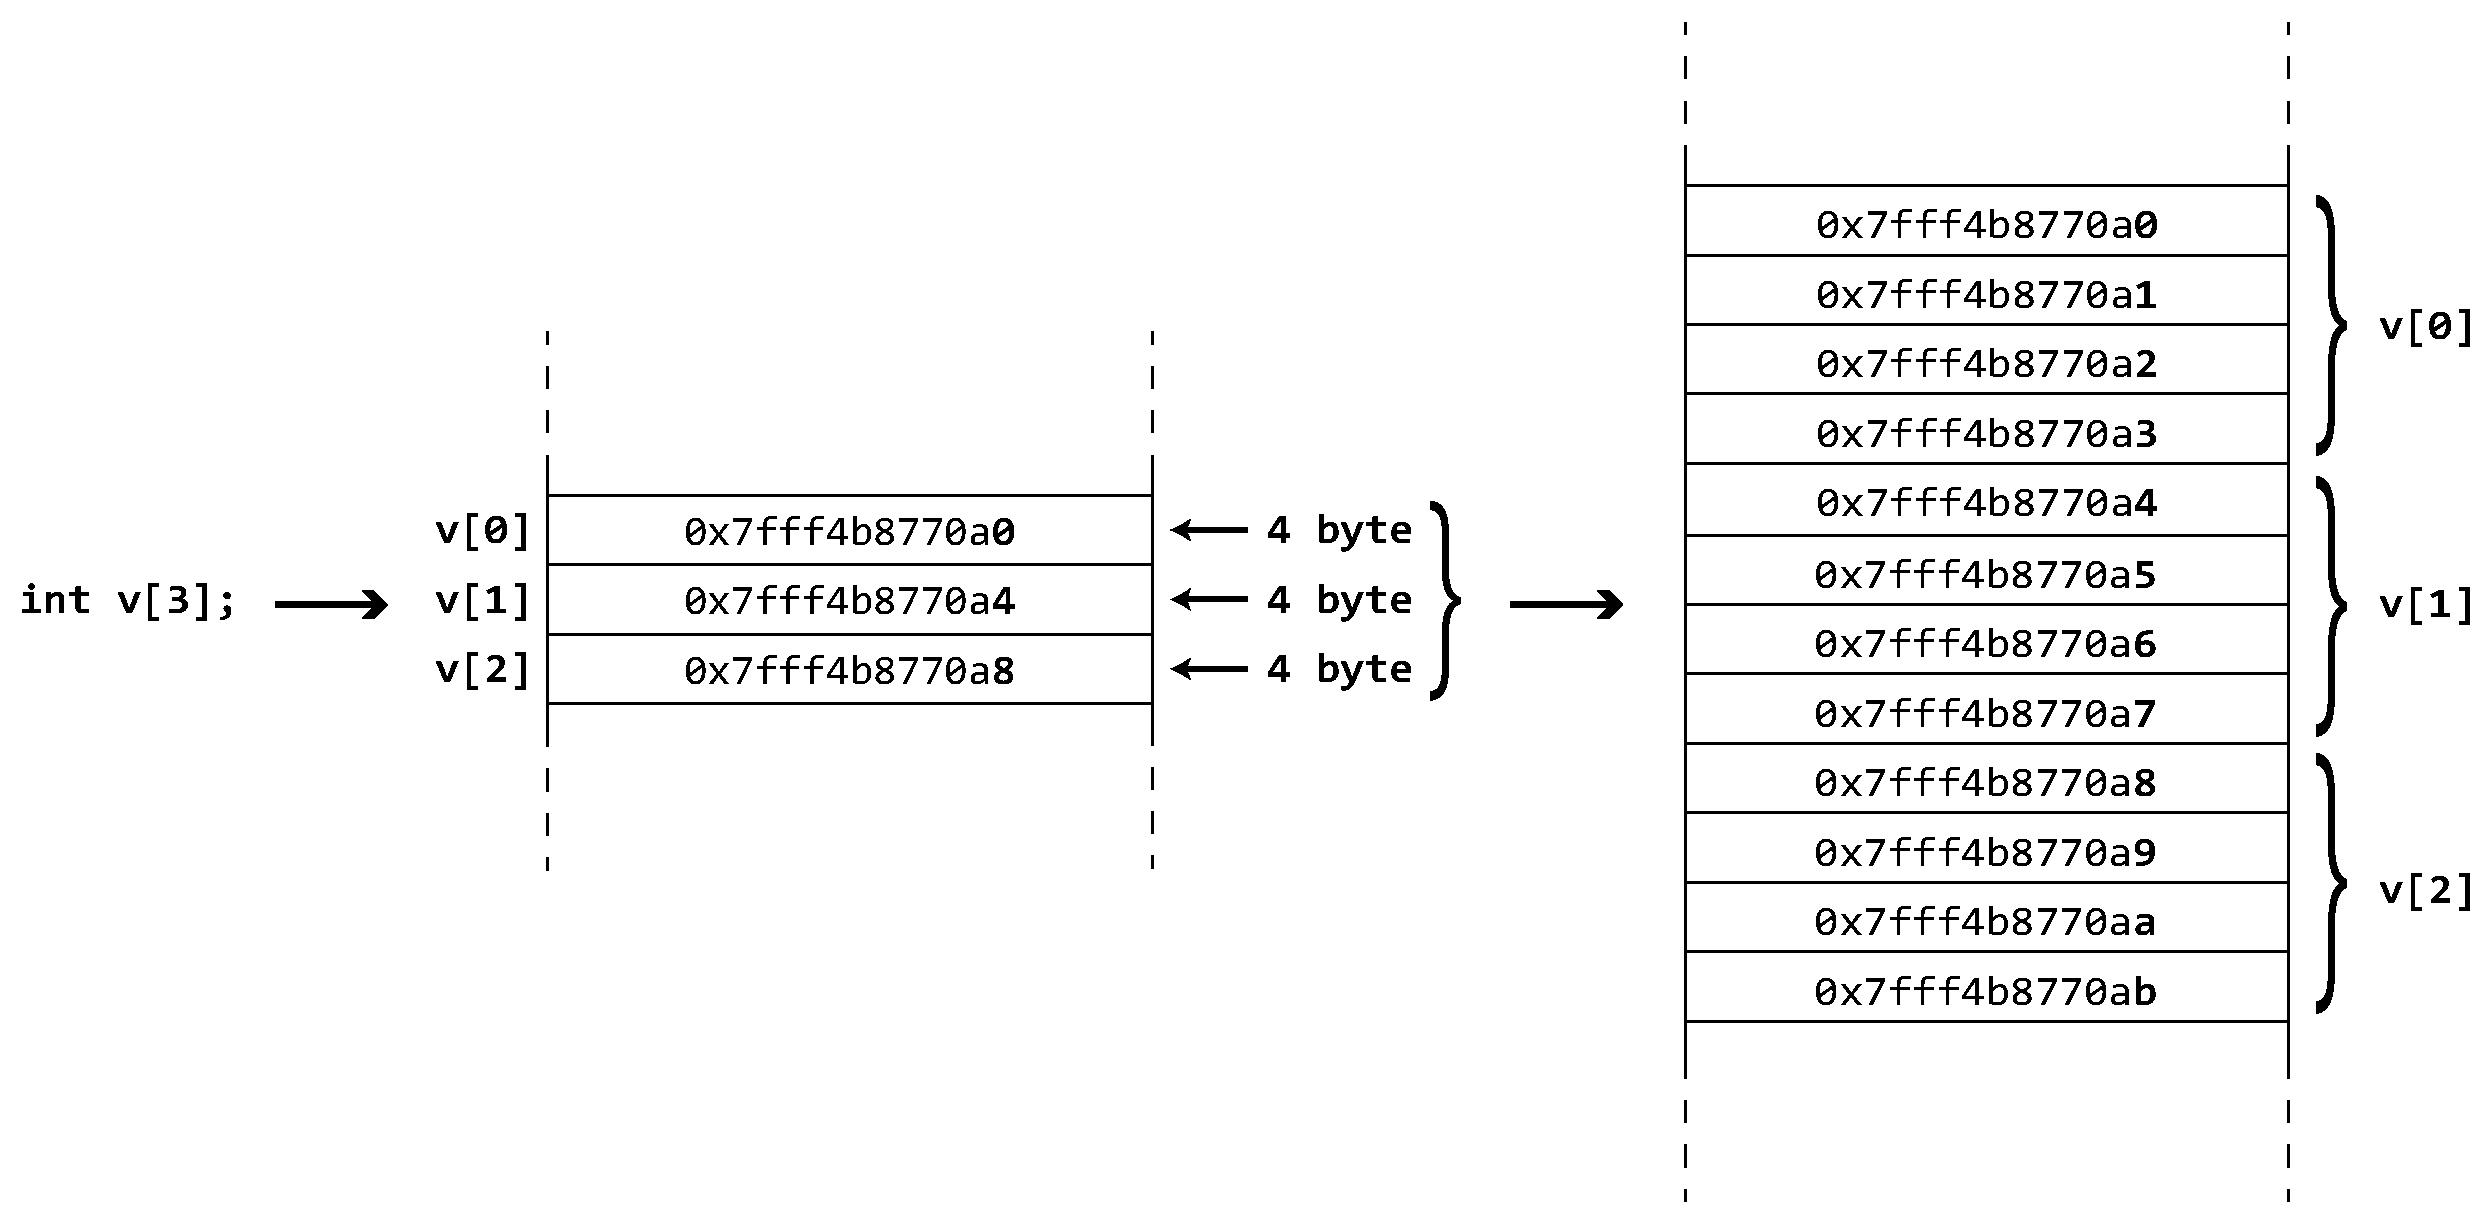
\includegraphics[scale=0.35]{Immagini/array_mem.pdf}  
	\captionsetup{margin=1.5cm} %justification=centering,
	\caption{Rappresentazione di un \emph{array} in memoria. La prima schematizzazione rappresenta gli elementi (\textbf{int}) dell'\emph{array} con i relativi indirizzi. La seconda schematizzazione rappresenta tutti i singoli byte dell'\emph{array}: notare che l'indirizzo di ogni elemento è l'indirizzo del suo primo byte.\protect\footnotemark}
	\label{memory2}
\end{figure}



	Una parte di un esercizio di un tema d'esame (25 febbraio 2014) chiedeva:
\begin{shaded}
Sia
 
\qquad\textbf{int} \verb|w[5];|\\
se l'indirizzo di \verb|w[0]| termina con \verb|1dfd| come terminano gli indirizzi 
di \verb|w[2]| e \verb|w[4]|?
\end{shaded}
Per trovare l'indirizzo di \verb|w[2]|, dobbiamo sommare 8 byte all'indirizzo di \verb|w[0]|, e quindi troviamo $1e16$. Per trovare l'indirizzo di \verb|w[4]|, sommiamo altri 8 byte e troviamo $1e1a$.
\begin{subappendices}
	\section*{COMPLEMENTI}
	\addcontentsline{toc}{section}{COMPLEMENTI}
%\begin{small}
 \footnotetext{Ringrazio Stefano Balzan per la realizzazione dell'immagine.} %va messo qua per avere la nota nella stessa pagina dell'immagine... che schifo...
\section{Architetture a 32 e 64 bit}\label{archCPU}
Questa sezione, per programmare in \verb|C++|, non ha alcuna utilità  pratica, ma può essere interessante a livello ``culturale''.\\

Hai mai sentito parlare di computer a 32 e a 64 bit? 

Il processore comunica con la memoria tramite dei \emph{bus}, che sono veri e propri canali fisici della scheda madre: vi è il \emph{bus} degli indirizzi, il \emph{bus} dei dati e il \emph{bus} di controllo; quest'ultimo, a noi, non interessa. Nel \emph{bus} degli indirizzi viaggia l'indirizzo fisico a cui andare a leggere o scrivere, mentre nel \emph{bus} dei dati passa il dato letto o da scrivere. Ecco, la dicitura ``32 bit'' indica esattamente la dimensione di questi \emph{bus}, oltre alla dimensione di alcune piccolissime memorie interne alla CPU, detti \emph{registri} (la RAM, per la CPU, è lenta: i \emph{registri} sono piccolissime memorie ad accesso praticamente istantaneo utilizzate per scrivere i risultati intermedi di calcoli vari). L'insieme di queste caratteristiche costituisce l'\emph{architettura} della CPU. 

I primi computer avevano \emph{bus} da 8 bit, quindi da 16 (ad esempio Windows 95 era scritto per girare su computer di questo tipo). Poi si è passati a 32 e, più o meno recentemente, sono nate CPU a 64 bit, che oggi predominano il panorama.

Ma cosa cambia tra queste diverse architetture? 

La prima grande restrizione è nel \emph{bus} degli indirizzi. Torniamo alla fine degli anni '90, quando l'architettura maggiormente in voga era il 32 bit. Quanto è grande un indirizzo da 32 bit in base decimale? Una variabile di questa dimensione può immagazzinare numeri che vanno da 0 a 4.294.967.296. Se ogni numero rappresenta un indirizzo di memoria (e, ricorda, ogni indirizzo è un byte), posso indicizzare circa $4\cdot10^9$ byte, ovvero 4 gigabyte. Ecco trovato il primo limite dei 32 bit: un processore di questo tipo non può gestire una RAM più grande di 4 gigabyte\footnote{In realtà ben presto nacque la tecnologia PAE ("Phisical Address Extention") che aggiunge 4 bit agli indirizzi fisici: il sistema operativo riesce così a gestire fino a 64GB di memoria, ma i singoli programmi rimangono limitati a 4GB.}. 

L'altro limite riguarda il \emph{bus} di dati: anche le variabili sono limitate a 32 bit e una CPU di questo tipo non sa gestire in maniera naturale i \textbf{long} e i \textbf{double}.

Ben presto i 32 bit divennero eccessivamente limitanti e, nei primissimi anni duemila, nacque l'architettura a 64 bit:  il primo utilizzatore (e per un po' l'unico) fu Linux. Con i 64 bit la dimensione fisica di entrambi i \emph{bus} fu raddoppiata. Consideriamo gli indirizzi: $2^{64}$ è circa $1.8\cdot10^{19}$, ovvero circa 18 milioni di terabyte ($1.8\cdot10^{10}$ gigabyte, qualcosa di spropositato). Le prime versioni dell'architettura a 64 bit limitarono il \emph{bus} virtuale degli indirizzi a 48 bit: in questo modo sono indicizzabili 256 terabyte di RAM, assolutamente più che sufficienti oggi e, probabilmente, per molti altri anni\footnote{Alla data di scrittura, la maggior parte dei computer portatili sono dotati di 4-16 gigabyte di memoria, i server più potenti arrivano a 128.}.

I diversi sistemi operativi gestiscono questi indirizzi in maniera differente. Linux usa per i processi  47 bit di indirizzi rendendo utilizzabili ``solo'' 128TB (mentre il kernel li può usare tutti e 256). 

Windows, fino alla versione 7, limitava l'uso di solo 8TB di indirizzi virtuali. Dalla versione 8.1 è stato esteso l'uso a 128TB di indirizzi, ma purtroppo non esistono compilatori open-source a 64 bit (il compilatore proprietario Microsoft è a pagamento). Inoltre, a meno di non dare al compilatore l'opzione ``\emph{LARGEADDRESSAWARE}'', tutti i programmi sono limitati a 2 gigabyte (quindi anche meno dei 4GB delle  vecchie CPU da 32 bit\ldots). 

Per quanto riguarda MacOS, ammetto la mia completa ignoranza.

Tornando ai \emph{bus}, rimane da analizzare quello dei dati: a  differenza del \emph{bus} degli indirizzi, viene utilizzato interamente, permettendo di gestire in modo naturale dati da 8 byte (64 bit), cioè i nostri \textbf{long} e \textbf{double}. Ma non è l'unico vantaggio: l'esistenza delle piccole memorie interne alla CPU, anch'esse da 64 bit, permette di lavorare contemporaneamente su due dati da 4 byte (\textbf{float} e \textbf{int}) dimezzando il tempo di calcolo (se il codice macchina istruisce la CPU a farlo), ma questo interessa a chi scrive i compilatori\ldots.
%\end{small}

\end{subappendices}
